\documentclass{article}
% General document formatting
\usepackage[margin=0.7in]{geometry}
\usepackage[parfill]{parskip}
\usepackage[utf8]{inputenc}
\usepackage{tabularx}
\usepackage{graphicx}
\usepackage{subcaption}

% Related to math
% \usepackage{amsmath,amssymb,amsfonts,amsthm}
\pagenumbering{gobble}


\begin{document}
\newcolumntype{R}{>{\raggedleft\arraybackslash}X}

\noindent\begin{tabularx}{\textwidth}{XR}
  
\includegraphics[width=3cm]{./logo.jpg} & 
\includegraphics[width=3cm]{./cemvet.jpg} \\
\end{tabularx}


\begin{center}
  {\huge\textbf{Informe Ecográfico}}
\end{center}

\renewcommand{\arraystretch}{1.8}
\noindent\begin{tabularx}{\textwidth}{|XX|XX|}
  \hline
  \textbf{Paciente}           & Gatito  & \textbf{Especie} & Felino \\
  \hline
  \textbf{Ficha}              & 1234  & \textbf{Edad}    & 4 años \\
  \hline
  \textbf{Tutor}              & Fita  & \textbf{Sexo}    & Macho \\
  \hline
  \textbf{Médico solicitante} & Pia Chang  & \textbf{Estudio} & Abdominal \\
  \hline
\end{tabularx}
\renewcommand{\arraystretch}{1}

\textbf{Antecedentes:} Aumento marcado de enzimas hepáticas, baja de peso e hiporexia crónica.


\section*{Descripción}
\textbf{Nefrourinario}: Imagen vesical semipletórica, contenido anecoico, pared de grosor normal. Uretra abdominal sin contenido. Imagenes renales simétricas, relación córtico medular aumentadaa, límite cortico medular definido, ecogenicidad cortical y medular normal, bordes regulares. Pelvis renales normales.

\textbf{Reproductor}: Imagen prostática con leve aumento de tamaño (3,1 cm de largo), homogénea con múltiples estructuras de aspecto quístico de hasta 3 mm distribuídas en todo el parénquima.

\textbf{Bazo}: Imagen esplénica de tamaño normal, homogénea, sin lesiones focales.

\textbf{Adrenales}: Imagenes adrenales normales.

\textbf{Hepatobiliar}: Imagen hepática con moderada disminución de tamaño, bordes regulares y redondeados, parénquima hiperecoico, presentando masa isoecoica ovoide de 5 cm largo x 3,7 alto x 5,3 cm ancho, de distribución central/izquierda, irrigada, y que por la reducción en el tamaño hepático se ve ocupando gran parte de este. Patrón venoso normal, flujo portal varía con la respiración (desde 9 a 21 m/seg velocidad media). Vesícula biliar distendida por contenido anecoico y moderada cantidad de sedimento hiperecoico en pared dependiente, pared de grosor normal, sin signos obstructivos.

\textbf{Gastrointestinal}: Imagen gástrica sin contenido, pared de grosor normal. Imagen duodenal en patrón mucoso, pared de grosor normal. Imagen yeyunal en patrón mucoso, pared con engrosamiento difuso (3,6 mm). Imagen colónica con contenido de aspecto sólido, pared de grosor normal.

\textbf{Páncreas}: Páncreas levemente engrosado (1,6 cm ancho de lobo derecho), parénquima levemente hiperecoico y con estriaciones hipoecoicas. 

Linfonodos abdominales normales.

Pequeña cantidad de líquido libre anecoico perivesical, entre asas intestinales y craneal al higado.


\section*{Conclusiones}
Microhepatia moderada, parénquima de aspecto inflamatorio crónico, fibrótico o infiltrativo. Masa hepática según descripción, de aspecto neoproliferativo o compatible con gran nódulo de regeneración/hiperplasia, sugiero confirmación histopatológica. Barro biliar. Edema pancreático. Enteritis difusa.  Derrame peritoneal leve.  Nefropatía bilateral de aspecto inflamatorio agudo. Prostatomegalia de aspecto hiperplásico y múltiples quistes asociados.

\vfill

\begin{figure}[h]
\noindent Atte.
  \begin{flushright}

\includegraphics[width=3cm]{./firma.jpg} \\
Pia Chang \\
Médico Veterinario \\
Diploma en imagenología
\end{flushright}
9 de junio de 2019
\end{figure}

\renewcommand{\arraystretch}{4}

\noindent\begin{tabularx}{\textwidth}{XR}
  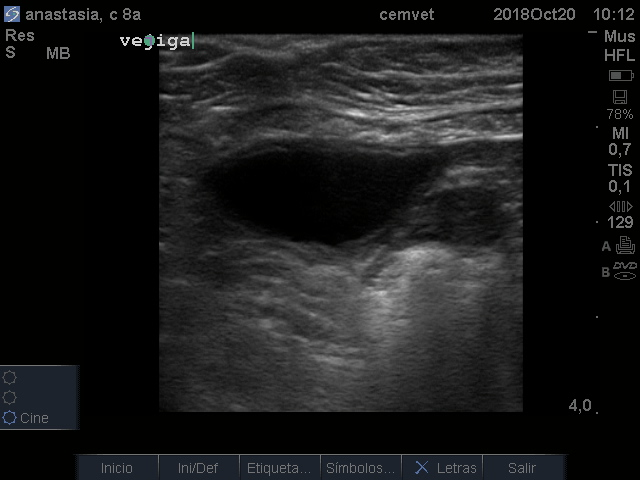
\includegraphics[width=8.5cm,trim={85px 45px 45px 25px},clip]{./example/101204hs[0048131].jpg} & 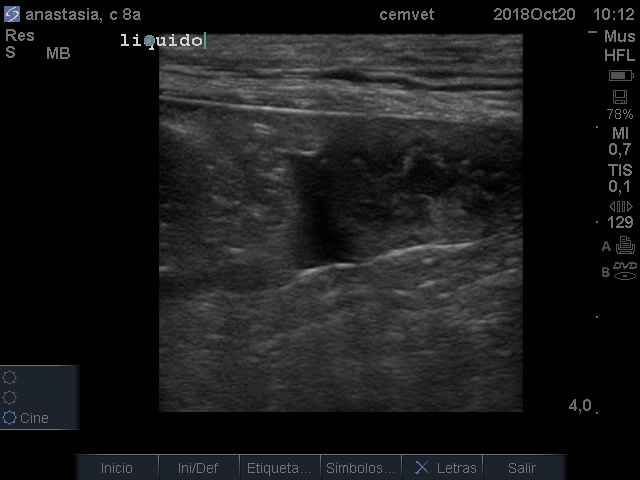
\includegraphics[width=8.5cm,trim={85px 45px 45px 25px},clip]{./example/101242hs[0048133].jpg} \\
\end{tabularx}

\noindent\begin{tabularx}{\textwidth}{XR}
  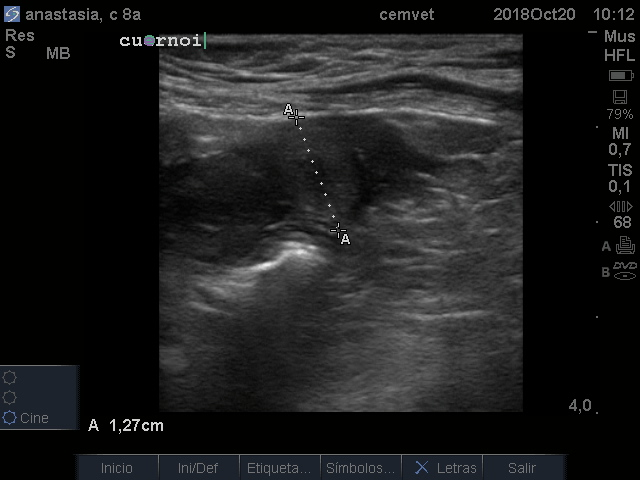
\includegraphics[width=8.5cm,trim={85px 45px 45px 25px},clip]{./example/101221hs[0048132].jpg} & 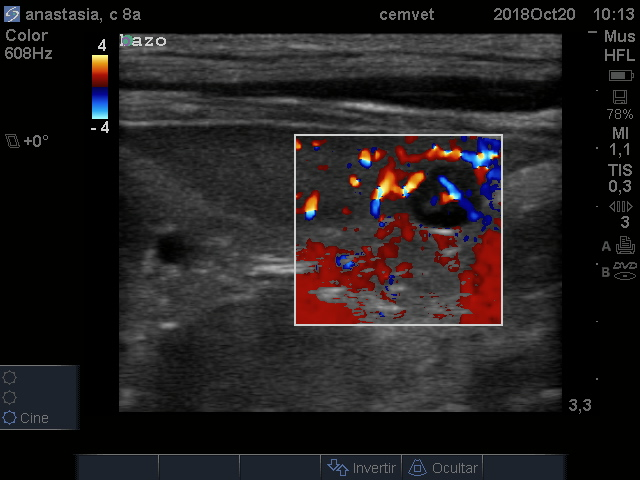
\includegraphics[width=8.5cm,trim={85px 45px 45px 25px},clip]{./example/101313hs[0048135].jpg} \\
\end{tabularx}

\noindent\begin{tabularx}{\textwidth}{XR}
  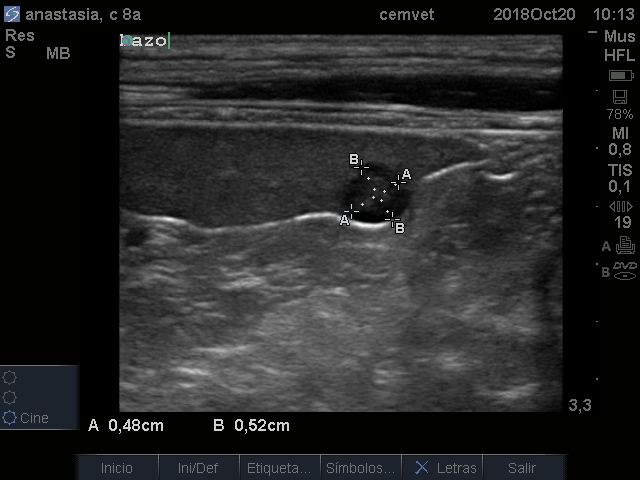
\includegraphics[width=8.5cm,trim={85px 45px 45px 25px},clip]{./example/101304hs[0048134].jpg} &  \\
\end{tabularx}

\renewcommand{\arraystretch}{1}

\end{document}